\chapter{Versuchsdurchführung}

\section{Versuchsaufgabe 1: Statische Messung der Diodenkennlinie}

Folgende Dioden werden untersucht:

\begin{itemize}
    \item{D1:} Silizium-Diode MRA4004, max. Sperrspannung $400 \si{\volt}$; max. Durchlassstrom $1000 \si{\milli\ampere}$;
    \item{D2:} Schottky-Diode 10BQ015, max. Sperrspannung $15 \si{\volt}$; max. Durchlassstrom $1000 \si{\milli\ampere}$.
\end{itemize}

Zur statischen Messung der Diodenkennlinie ($I = f(U)$) wird die Diode in Reihe mit einem Widerstand $R = 100 \si{\ohm}$ geschaltet.
In Durchlassrichtung der Dioden wird spannungsrichtig gemessen (siehe Voraufgabe F):
Die Spannung $U$ wird dabei nur über die Diode mit dem analogen Messgerät (UNIGOR 4P) gemessen, 
der Strom $I$ hingegen mit dem digitalen Multimeter (DMM), aufgrund dessen schlechteren Genauigkeit.

In Sperrrichtung wird umgekehrt verfahren: Für die stromrichtige Messung wird die Spannung $U$ über Diode und analogem Amperemeter gemessen,
der Strom $I$ hingegen mit dem DMM.

% Schaltungsskizze?

Aus unserer Messung bei geeigneten ausgewählten Spannungswerten ergeben sich folgende Kennlinien:
% Plots
% Auswertung


\section{Versuchsaufgabe 2: Oszillogramm der Diodenkennlinie}

Nun soll die Kennlinie der Diode mit einem Oszilloskop aufgenommen werden.
Dies wird umgesetzt, indem eine Wechselspannung an die Diode angelegt wird, 
die dann in Durchlassrichtung und Sperrrichtung abwechselnd wirkt.
Um den Strom, der durch die Diode fließt, zu messen, wird mithilfe der Black Box die Spannung vor und nach dem Widerstand $R = 100 \si{\ohm}$
zu einem Referenzpotential gemessen (siehe \ref{fig:2_strom}).

\begin{figure}[H]
    \centering
    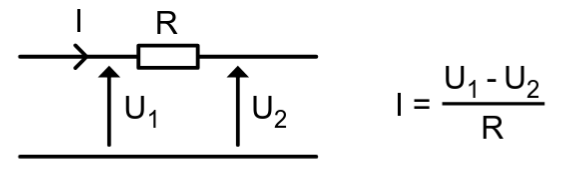
\includegraphics[width=0.5\textwidth]{figs/2/strom.png}
    \caption{Zur Strommessung}
    \label{fig:2_strom}
\end{figure}

Dadurch erhält man als Ausgang eine Spannung, die proportional zum Strom $I$ ist, der durch die Diode fließt.
Betrachtet man nun diese Spannung und die Eingangswechselspannung am Oszilloskop im XY-Modus, und steigert die Amplitude der Wechselspannung,
so erscheint die Kennlinie der Diode als Oszillogramm.

% Schaltungsskizze?

Zusätzlich zu den Dioden D1 und D2 wird jetzt auch eine Zener-Diode ZD untersucht.
Es ergeben sich folgende Kennlinien:

\begin{figure}[H]
    \centering
    \begin{subfigure}[b]{0.45\textwidth}
        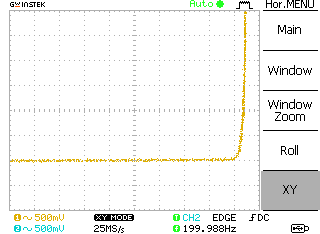
\includegraphics[width=\textwidth]{figs/2/DS0000.png}
        \caption{D1}
        \label{fig:2_D1}
    \end{subfigure}
    \hfill
    \begin{subfigure}[b]{0.45\textwidth}
        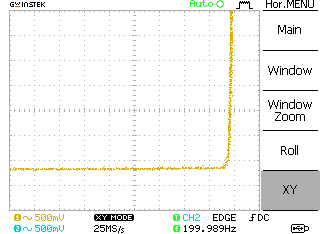
\includegraphics[width=\textwidth]{figs/2/DS0001.png}
        \caption{D2}
        \label{fig:2_D2}
    \end{subfigure}
    \vspace{0.5em}
    \begin{subfigure}[b]{0.45\textwidth}
        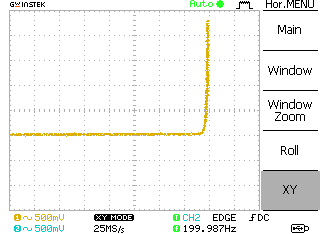
\includegraphics[width=\textwidth]{figs/2/DS0002.png}
        \caption{ZD}
        \label{fig:2_ZD_1}
    \end{subfigure}
    \hfill
    \begin{subfigure}[b]{0.45\textwidth}
        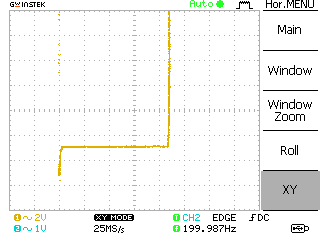
\includegraphics[width=\textwidth]{figs/2/DS0003.png}
        \caption{ZD in größerem Bereich}
        \label{fig:2_ZD_2}
    \end{subfigure}
    \caption{Oszillogramme der Diodenkennlinien}
\end{figure}


Die charakteristischen Kennlinien der Dioden sind zu erkennen. 
Man erkennt, dass die Schottky-Diode D2 eine leicht geringere Durchlassspannung (ca. $\SI{1,8}{\volt}$) aufweist als die Silizium-Diode D1 (ca. $\SI{2,0}{\volt}$).
Die der Zener-Diode ZD ist mit ca. $\SI{1,3}{\volt}$ noch einmal deutlich geringer.
Es fällt auf, dass diese Werte nicht nah am erwarteten Wert von $\SI{0,6}{\volt}$ liegen.
Außerdem fällt auf, dass die Kennlinien in den konstanten Bereichen nicht auf 0 sind, 
obwohl wir mit einer sehr niedrigen Wechselspannung von ca. $\SI{20}{\milli\volt}$ verifiziert hatten, dass der Nullpunkt im Ursprung des Oszilloskops liegt.
Während unserer Aufzeichnung konnten wir verstellen, dass durch die kontinuierliche Änderung der Spannung die Kennlinie sich nach unten und rechts (??) verschiebt,
also sowohl in $x$- als auch in $y$-Richtung.
Dies erklärt auch die Abweichung der Durchlassspannung von den erwarteten Werten.
Dieses Phänomen konnten wir auch bei anderen Komilitonen unserer Gruppe beobachten. 
Es scheint also ein generelles Problem zu sein, das nicht nur auf unsere Messung zurückzuführen ist.
Die Ursache hierfür ist uns nicht bekannt.
% AI AM KOCHEN
% , aber es könnte an der Black Box liegen, die wir für die Messung verwendet haben.
% Die Black Box könnte eine gewisse Eigenkapazität besitzen, die die Spannung beeinflusst, die wir messen.
% Eine weitere Möglichkeit wäre, dass die Black Box nicht für Wechselspannungen geeignet ist, 
% sondern nur für Gleichspannungen, und die Messung daher nicht korrekt ist.

Als Zenerspannung erhalten wir einen abgelesenen Wert von $(2,9 \pm 0,1)\si{\volt}$ (Unsicherheit abgeschätzt).